\cleardoublepage

\chapter{}
\label{chap:a}

\begin{description}[leftmargin=!,labelwidth=\widthof{\bfseries Volume and number}]
    \item[Title] Assessment of Incident Power Density on Spherical Head Model up to 100 GHz
    \item[Authors] Ante Kapetanović, Dragan Poljak
    \item[Journal] IEEE Transactions on Electromagnetic Compatibility
    \item[Year] 2022
    \item[Volume and number] 64, 5
    \item[Pages] 1296--1303
    \item[Categorization] Research paper
    \item[Language] English
    \item[Keywords] compliance assessment, human head, incident power density, millimeter waves, radiation safety
    \item[Abstract] This article presents a technique for the accurate assessment of the spatially averaged incident power density (IPD) on a spherical human head model from 3.5 to 100 GHz.
    The spatially-averaged IPD is defined either by averaging components of the power density vector normal to an evaluation surface, or by averaging its norm.
    The electromagnetic exposure assessment is provided for a dipole antenna placed at a separation distance of 2--150 mm from the model.
    We compare the IPD averaged over a proposed spherical surface with differently positioned planar surfaces.
    Results show that, for appropriate settings of the exposure above 6 GHz, the IPD averaged on a spherical surface is up to 12\% larger for the normal definition, while marginally lower for the norm definition.
    In the worst case scenario, the spatially averaged IPD on a spherical surface is up to about 30\% larger regardless of the definition.
    Comparative analysis between the definitions of the IPD averaged on a spherical model demonstrates that the norm definition yields significantly larger values in the reactive near field at characteristic frequencies, whereby this difference is marginal out of the reactive near field.
    \item[Databases] Scopus, Google Scholar, Web of Science Core Collection -- Science Citation Index Expanded
    \item[Impact factor] 2.036
    \item[DOI] \href{https://doi.org/10.1109/TEMC.2022.3183071}{\url{10.1109/TEMC.2022.3183071}}
    \item[Copyright notice] \copyright 2022 IEEE. Reprinted, with permission, from Ante Kapetanović and Dragan Poljak, Assessment of Incident Power Density on Spherical Head Model up to 100 GHz, IEEE Transactions on Electromagnetic Compatibility, 2022
\end{description}

\cleardoublepage

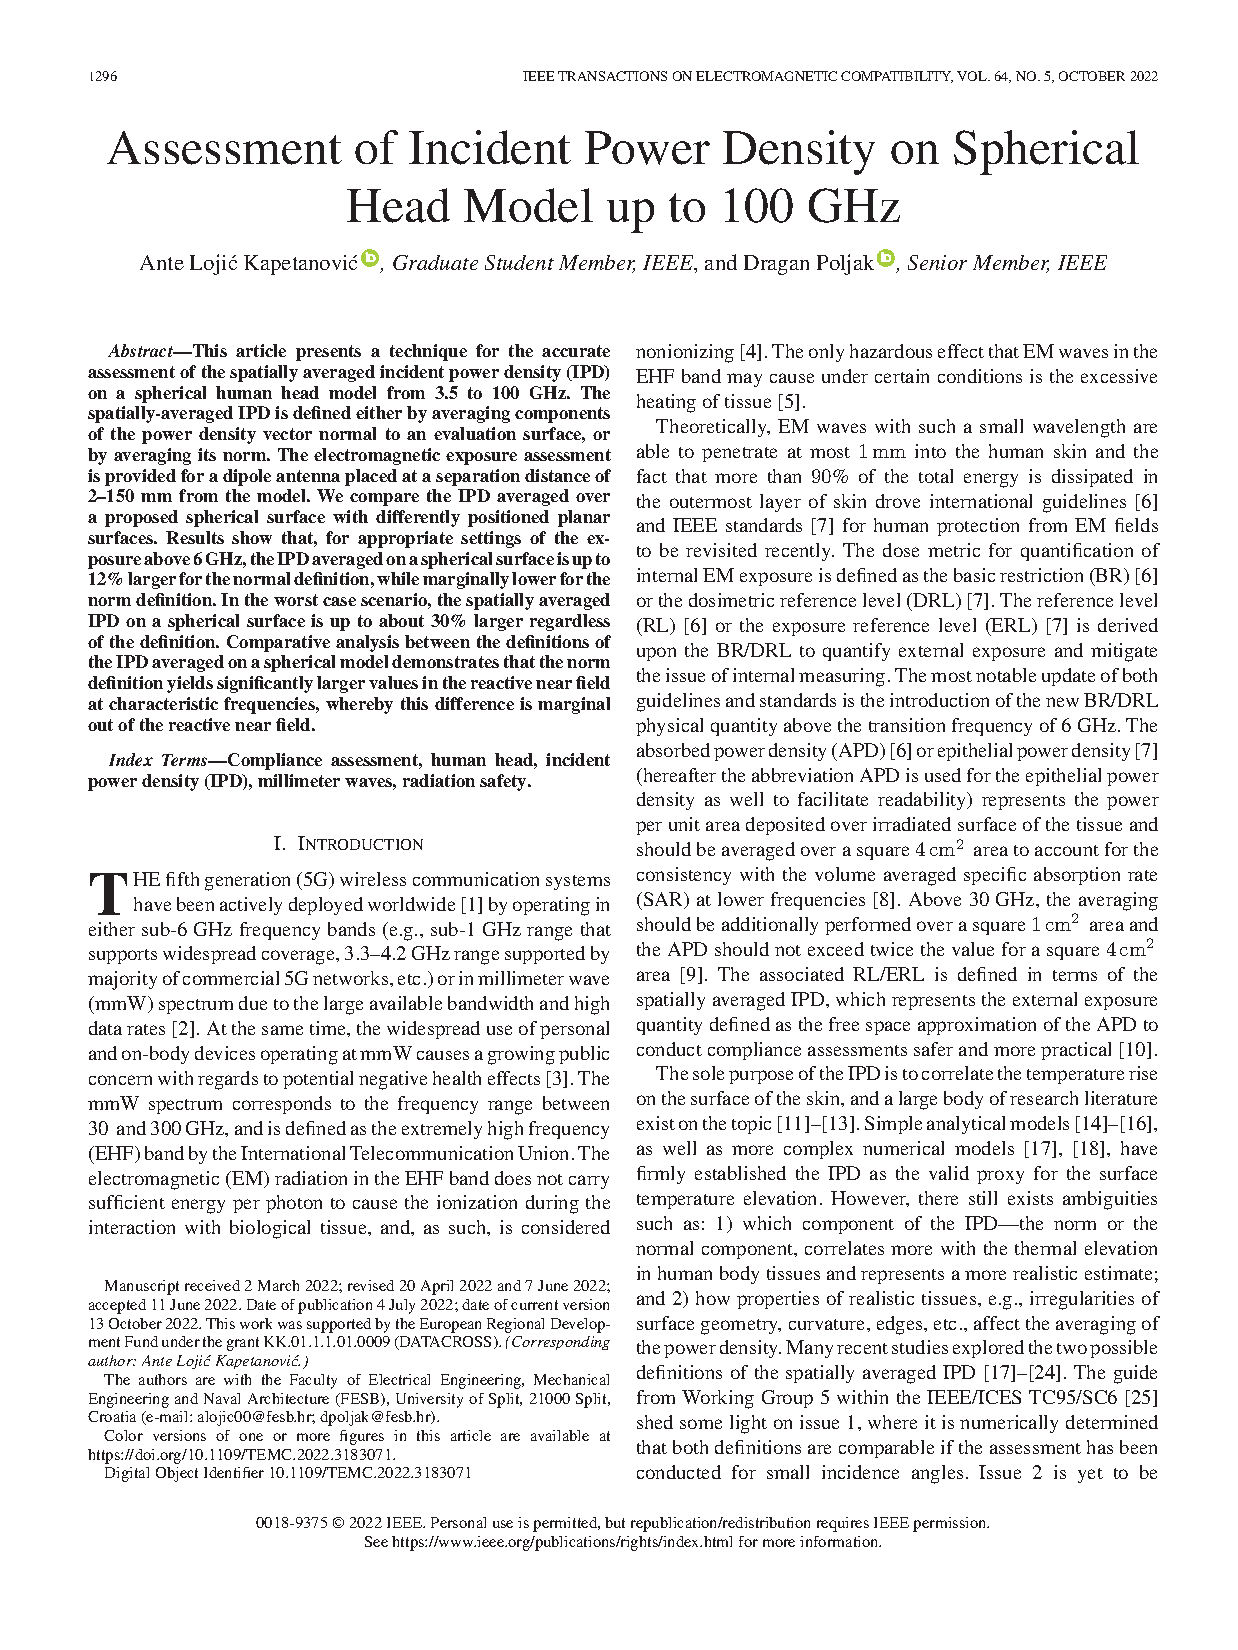
\includepdf[pages=-, pagecommand={\thispagestyle{includepdfstyle}}]{papers/Kapetanovic2022temc.pdf}
